\documentclass[11pt,paper=letter]{scrartcl}
\usepackage[alttitle]{cjquines}

\setlength{\oddsidemargin}{0.8in}
\setlength{\evensidemargin}{0.8in}
\setlength{\textwidth}{6.9in}
\setlength{\textheight}{8.5in}
\setlength{\headheight}{0pt}
\setlength{\headsep}{15pt}

\pretitle{\vspace{-6em} \begin{flushleft} \bfseries \Large}
\posttitle{\vspace{-0.6em} \end{flushleft}}
\preauthor{\begin{flushleft} \itshape \Large}
\postauthor{\vspace{-0.7em} \end{flushleft}}
\predate{\begin{flushleft} \Large}
\postdate{\end{flushleft} \rule{\textwidth}{0.5pt}}

\begin{document}

This is the practice test, due on Friday, October 27, 2017.

\begin{itemize}
  \item The test follows the qualifying stage format, which means the time limit is two hours. These should be continuous; do not work for one hour on one day and then one hour on another day.
  \item No aids except scratch paper, ruler, and compass are permitted. No graph paper, protractors, calculators, computers, or mobile phones are allowed. Do not leave the testing area for the duration of the exam.
  \item Write your answers legibly on a clean sheet of short bond paper, with your name.
  \item Do not discuss the problems before Friday, October 27, when they are due.
\end{itemize}

\noindent
\textbf{Do not turn the page} until you have a timer for two hours and are ready to answer \textbf{without interruptions}. 

\newpage

\title{$\qquad\qquad\qquad$ Program for Inducing Mathematical Excellence}
\author{$\qquad\qquad\qquad\;\;\,$ Practice Final Exam}
\date{$\qquad\qquad\qquad\quad$ 27 October 2017}

\maketitle
\setlength{\unitlength}{1in}
\begin{picture}(0,0)
  \put(0.1,0.6){\hbox{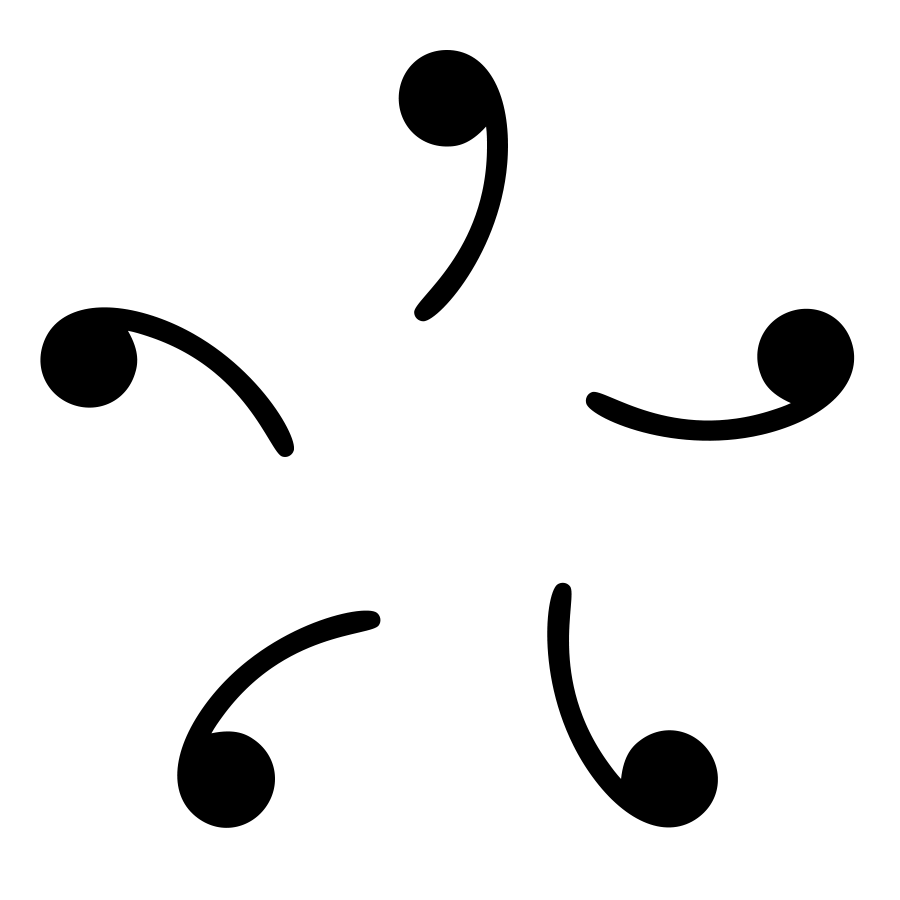
\includegraphics[width=0.9in]{logo.png}}}
\end{picture}
\vspace{-2em}

\noindent\textbf{PART I.} Choose the best answer. Each correct answer is worth two points.

\begin{enumerate}
  \item Let $m$ be a positive integer less than $2015$. What is the largest possible remainder when $2015$ is divided by $m$?

  \fourch
  {$1004$}
  {$1005$}
  {$1006$}
  {$1007$}

  \item Compute $\sqrt{(31)(30)(29)(28) + 1}$.

  \fourch
  {$701$}
  {$755$}
  {$811$}
  {$869$}

  \item Three fair six-sided dice are labeled $\cbr{1,2,3,4,5,6}$, $\cbr{1,2,3,4,5,6}$, and $\cbr{1,2,3,7,8,9}$. All three dice are rolled. What is the probability that at least two have the same value?

  \fourch
  {$\dfrac14$}
  {$\dfrac5{18}$}
  {$\dfrac{11}{36}$}
  {$\dfrac13$}

  \item Suppose $w, x, y, z$ are real numbers greater than $1$ such that $\log_x w = 24, \log_y w = 40$ and $\log_{xyz} w = 12$. Find $\log_z w$.

  \fourch
  {$15$}
  {$30$}
  {$60$}
  {$120$}

  \item Let $ABCD$ be a square with side length $100$, and let $M$ be the midpoint of $AB$. Point $P$ is selected inside $ABCD$ such that $MP = 50$ and $PC = 100$. Find $AP^2$.

  \fourch
  {$1400$}
  {$1600$}
  {$1800$}
  {$2000$}

  \item Let the four real solutions to the system $x^2 + 6y - 36 = 0$ and $y^2 - 6x - 36 = 0$ be $(x_1, y_1)$, $(x_2, y_2)$, $(x_3, y_3)$ and $(x_4, y_4)$. What is $\del{y_1 + y_2 + y_3 + y_4} - \del{x_1 + x_2 + x_3 + x_4}$?

  \fourch
  {$0$}
  {$6$}
  {$18$}
  {$36$}

  \item There exists three-digit numbers $A$, $B$ and $C$ such that moving the last digit of $A$ to its beginning gives $B$, and moving the last digit of $B$ to its beginning gives $C$. Both $A$ and $B$ are perfect squares, but $C$ is not. What is the sum of $C$'s digits, given it is not a perfect square?

  \fourch
  {$7$}
  {$10$}
  {$13$}
  {$16$}

  \item What is the sum of the coefficients in the expansion of $(x+y)^{10} + (x-y)^{10}$?

  \fourch
  {$512$}
  {$513$}
  {$1024$}
  {$1025$}

  \item What are the last two digits of $11^{2401}$?

  \fourch
  {$11$}
  {$31$}
  {$51$}
  {$71$}

  \item The \emph{hotel elevator cubic} polynomial $P(x)$ satisfies $P(11) = 11$, $P(12) = 12$, $P(13) = 14$ and $P(14) = 15$. What is $P(15)$?

  \fourch
  {$13$}
  {$14$}
  {$15$}
  {$16$}

  \item The common external tangent of two circles has length $2017$ and their common internal tangent has length $2009$. What is the product of their radii?

  \fourch
  {$8040$}
  {$8044$}
  {$8048$}
  {$8052$}

  \item Find the sum of all positive rational numbers less than $10$ with denominator $30$ when written in lowest terms.

  \fourch
  {$373$}
  {$381$}
  {$390$}
  {$400$}

  \item How many positive integers divide at least two of the numbers $120$, $144$, and $180$?

  \fourch
  {$11$}
  {$13$}
  {$15$}
  {$17$}

  \item Let $2000 < N < 2100$ be an integer. The last day of year $N$ is a Tuesday and the first day of year $N+2$ is a Friday. The fourth Sunday of year $N+3$ is the $m$th day of January. What is $m$?

  \fourch
  {$23$}
  {$25$}
  {$27$}
  {$29$}

  \item In square $ABCD$ with area $1$, points $A', B', C'$ and $D'$ are on $BC, CD, DA$ and $AB$ respectively, such that $A'C = B'D = C'A = D'B = 1/n$, for some $n$. The lines $AA', BB', CC'$ and $DD'$ construct a small square with area $1/1985$. Find $n$.

  \fourch
  {$28$}
  {$30$}
  {$32$}
  {$35$}
\end{enumerate}

\vspace{1em}
\noindent\textbf{PART II.} Choose the best answer. Each correct answer is worth three points.

\begin{enumerate}
  \item An arithmetic sequence of positive integers is called \emph{gleaming} if it has at least three terms, exactly one of which is larger than $2017$. Find the remainder when the number of gleaming sequences is divided by $1000$.

  \fourch
  {$136$}
  {$272$}
  {$408$}
  {$544$}

  \item Let $\mathcal S$ be a set of positive integers such that $1$ is in $\mathcal S$, and for all integers $n > 1$, an even number of divisors of $n$ are in $\mathcal S$. Find the $50$th smallest positive integer not in $\mathcal S$.

  \fourch
  {$118$}
  {$123$}
  {$128$}
  {$133$}

  \item Convex pentagon $ABCDE$ satisfies $AB \parallel DE$, $BE \parallel CD$, $BC \parallel AE$, $AB = 30$, $BC = 18$, $CD = 17$, and $DE = 20$. Find its area.

  \fourch
  {$612$}
  {$624$}
  {$636$}
  {$648$}

  \item The first three terms of an increasing geometric series are $x, y, z$, all positive integers. Given $1 + \log_2\del{xy+z} = \log_2\del{xz+y}$, find the minimum possible value of $x+y+z$.

  \fourch
  {$50$}
  {$55$}
  {$60$}
  {$65$}

  \item Let $P(n)$ be the product of the non-zero digits of $n$. Find the largest prime factor of the sum $P(1) + P(2) + \cdots + P(999)$.

  \fourch
  {$97$}
  {$101$}
  {$103$}
  {$107$}

  \item Find the $50$th smallest positive integer whose base two representation has an equal number of zeroes and ones. (For example, the smallest numbers with this property are $10_2$, $1001_2$, $1010_2$, and $1100_2$.)

  \fourch
  {$228$}
  {$232$}
  {$240$}
  {$527$}

  \item Find the greatest positive integer $n$ such that $2^n$ divides $\text{lcm}\left(1^1,2^2,3^3,\ldots,2016^{2016}\right).$

  \fourch
  {$10240$}
  {$13440$}
  {$13824$}
  {$14336$}

  \item Let $a$, $b$, and $c$ be the roots of $2x^3-x^2+3x-2 \cdot 3$. Find the value of $\sqrt{a^2+3} \cdot \sqrt{b^2+3} \cdot \sqrt{c^2+3}$.

  \fourch
  {$2$}
  {$3$}
  {$6$}
  {$8$}

  \item In triangle $ABC$, let ${AB}=14$, ${BC}=15$, and ${CA}=13$. Let $D$ be the foot of the altitude from $C$ to ${AB}$, $M$ be the midpoint of ${AB}$, and $N$ be the midpoint of ${DM}$. Find the length of ${CN}$.

  \fourch
  {$\sqrt{145}$}
  {$7\sqrt{3}$}
  {$5\sqrt{6}$}
  {$\sqrt{155}$}

  \item A strictly increasing arithmetic sequence $a_1, a_2, a_3, \ldots, a_{100}$ of positive integers satisfies \[a_1+a_4+a_9+\cdots+a_{100}=\text{1000},\] where the summation runs over all terms of the form $a_{i^2}$ for $1\leq i\leq 10$. Find $a_{50}$.

  \fourch
  {$118$}
  {$123$}
  {$128$}
  {$133$}
\end{enumerate}

\newpage
\noindent\textbf{PART III.} All answers should be in simplest form. Each correct answer is worth six points.

\begin{enumerate}
  \item Find the value of $$\frac{1}{0! + 1!} + \frac{1}{1! + 2!} + \frac{1}{2! + 3!} + \frac{1}{3! + 4!} + \cdots .$$
  \item Find the sum of all positive integers $n$ such that exactly $2\%$ of the numbers in the set $\{1, 2, \ldots, n\}$ are perfect squares.
  \item Let $\triangle ABC$ be a triangle with $AB = 3$ and $AC = 5$, and suppose there exists a point $P$ on line $BC$ satisfying $AP \cdot BC = BP \cdot AC = CP \cdot AB.$ Find the product of all possible values of $BC^2$.
  \item A word is constructed out of five letters $A, B, C, D, E$ and is compressed in the following way: each consecutive string of identical letters is replaced with the length of the string and the letter used. For example, $ABBACCCAA$ is compressed to $1A2B1A3C2A$. Find the expected value of the length of the compressed form of a randomly selected nine-letter word.
  \item Let $a, b, c, d, e,$ and $f$ be real numbers. Define the polynomials \[
 P(x) = 2x^4 - 26x^3 + ax^2 + bx + c \quad\text{ and }\quad Q(x) = 5x^4 - 80x^3 + dx^2 + ex + f. \] Let $S$ be the set of all complex numbers which are a root of either $P$ or $Q$ (or both). Given that $S = \{1,2,3,4,5\}$, compute $P(6) \cdot Q(6).$
\end{enumerate}

\end{document}
